%%
%% This is file `sample-sigconf.tex',
%% generated with the docstrip utility.
%%
%% The original source files were:
%%
%% samples.dtx  (with options: `sigconf')
%%
%% IMPORTANT NOTICE:
%%
%% For the copyright see the source file.
%%
%% Any modified versions of this file must be renamed
%% with new filenames distinct from sample-sigconf.tex.
%%
%% For distribution of the original source see the terms
%% for copying and modification in the file samples.dtx.
%%
%% This generated file may be distributed as long as the
%% original source files, as listed above, are part of the
%% same distribution. (The sources need not necessarily be
%% in the same archive or directory.)
%%
%% The first command in your LaTeX source must be the \documentclass command.
\documentclass[sigconf,review,anonymous]{acmart}

% Packages
\usepackage{amsfonts}
\usepackage{graphicx}
\usepackage{hyperref}
\usepackage{float}
\usepackage{pgfplots}
\usepgfplotslibrary{fillbetween}
\usepackage[pdf]{graphviz}
\usepackage{tikz}
\usepackage{natbib}
\usepackage{enumitem}

\usepackage{booktabs}
\usepackage{pifont}
\usepackage{fontawesome}

\newcommand{\wmark}{\textcolor{orange}{\ding{45}}}
\newcommand{\cmark}{\textcolor{green!80!black}{\ding{51}}}
\newcommand{\xmark}{\textcolor{red}{\ding{55}}}

\usepackage{multicol}

% Packages
\usepackage{amsmath}
\usepackage{soul}
\usepackage{listings}
\usepackage{xcolor}
\DeclareRobustCommand{\hlred}[1]{{\sethlcolor{pink}\hl{#1}}}
\usepackage{fontspec}

\setmonofont{JetBrainsMono}[
  Contextuals={Alternate},
  Path=./JetbrainsFontFiles/,
  Extension = .ttf,
  UprightFont=*-Regular,
  BoldFont=*-Bold,
  ItalicFont=*-Italic,
  BoldItalicFont=*-BoldItalic
]

\makeatletter
\def\verbatim@nolig@list{}
\makeatother

\lstdefinelanguage{kotlin}{
  comment=[l]{//},
  commentstyle={\color{gray}\ttfamily},
  emph={delegate, filter, firstOrNull, forEach, it, lazy, mapNotNull, println, repeat, assert, with, head, tail, len, return@},
  numberstyle=\noncopyable,
  emphstyle={\color{OrangeRed}},
  identifierstyle=\color{black},
  keywords={abstract, actual, as, as?, break, by, class, companion, continue, data, do, dynamic, else, enum, expect, false, final, for, fun, get, if, import, in, infix, interface, internal, is, null, object, open, operator, override, package, private, public, return, sealed, set, super, suspend, this, throw, true, try, catch, typealias, val, var, vararg, when, where, while, tailrec, reified},
  keywordstyle={\color{NavyBlue}\bfseries},
  morecomment=[s]{/*}{*/},
  morestring=[b]",
  morestring=[s]{"""*}{*"""},
  ndkeywords={@Deprecated, @JvmField, @JvmName, @JvmOverloads, @JvmStatic, @JvmSynthetic, Array, Byte, Double, Float, Boolean, Int, Integer, Iterable, Long, Runnable, Short, String},
  ndkeywordstyle={\color{BurntOrange}\bfseries},
  sensitive=true,
  stringstyle={\color{ForestGreen}\ttfamily},
  literate={`}{{\char0}}1,
  escapeinside={(*@}{@*)}
}

\lstset{basicstyle=\ttfamily\lst@ifdisplaystyle\small\fi}

%% NOTE that a single column version may be required for
%% submission and peer review. This can be done by changing
%% the \doucmentclass[...]{acmart} in this template to
%% \documentclass[manuscript,screen]{acmart}
%%
%% To ensure 100% compatibility, please check the white list of
%% approved LaTeX packages to be used with the Master Article Template at
%% https://www.acm.org/publications/taps/whitelist-of-latex-packages
%% before creating your document. The white list page provides
%% information on how to submit additional LaTeX packages for
%% review and adoption.
%% Fonts used in the template cannot be substituted; margin
%% adjustments are not allowed.
%%
%%
%% \BibTeX command to typeset BibTeX logo in the docs
\AtBeginDocument{%
  \providecommand\BibTeX{{%
    \normalfont B\kern-0.5em{\scshape i\kern-0.25em b}\kern-0.8em\TeX}}}

%% Rights management information.  This information is sent to you
%% when you complete the rights form.  These commands have SAMPLE
%% values in them; it is your responsibility as an author to replace
%% the commands and values with those provided to you when you
%% complete the rights form.
\setcopyright{acmcopyright}
\copyrightyear{2022}
\acmYear{2022}
\acmDOI{10.1145/1122445.1122456}

%% These commands are for a PROCEEDINGS abstract or paper.


\acmConference[ICSE 2022]{The 44th International Conference on Software Engineering}{May 21–29, 2022}{Pittsburgh, PA, USA}


\newcommand{\seqWord}{Seq \langle Word \rangle}
\newcommand{\distSeqWord}{Dist\langle \seqWord  \rangle}

\begin{document}

  \title{How robust is neural code completion to cosmetic variance?}
  \author{Breandan Considine, Xujie Si, Jin L.C. Guo}
  \email{breandan.considine@mail.mcgill.ca, {xsi, jguo}@cs.mcgill.ca}
  \affiliation{%
    \institution{McGill University}
  }

  \begin{abstract}
    Neural language models hold great promise as tools for computer-aided programming, but questions remain over their reliability and the consequences of overreliance. In the domain of natural language, prior work has revealed these models can be sensitive to naturally-occurring variance and malfunction in unpredictable ways. A closer examination of neural language models is needed to understand their behavior in programming-related tasks. In this work, we develop a methodology for systematically evaluating neural code completion models using common source code transformations such as synonymous renaming, intermediate logging, and independent statement reordering. Applying these synthetic transformations to a dataset of handwritten code snippets, we evaluate three SoTA models, CodeBERT, GraphCodeBERT and RobertA-Java, which exhibit varying degrees of robustness to cosmetic variance. Our approach is implemented and released as a modular and extensible toolkit for evaluating code-based neural language models.
  \end{abstract}

  \maketitle

  \section{Introduction}\label{sec:introduction}

  Neural language models play an increasingly synergetic role in software engineering, and are featured prominently in recent work on neural code completion~\cite{chen2021evaluating}. Yet from a development perspective, the behavior of these models is opaque: partially completed source code written inside an editor is sent to a remote server, which returns a completion. This client-server architecture can be seen as a black-box or \textit{extensional} function. Could there be a way to evaluate the behavior of neural language models in this setting?

  First conceived in the software testing literature, metamorphic testing~\cite{chen1995metamorphic} is a concept known in machine learning as \textit{self-supervision}. In settings where labels are scarce but invariant to certain groups of transformation or \textit{metamorphic relations}, given a finite labeled dataset, one can generate an effectively limitless quantity of synthetic data by selecting and recombining those transformations. For example, computer vision models should be invariant to shift, scale and rotation: given a small dataset of labeled images, we can apply these transformations to generate much larger training or validation set. Could similar kinds of transformations exist for code?

  Recent work in neural language modeling has shown impressive progress in long-range sequence prediction, starting with self-attention~\citep{vaswani2017attention}, to the BERT~\citep{devlin2018bert} and RoBERTa~\citep{liu2019roberta} architectures, now widely available in neural code completion models such as CodeBERT~\citep{feng2020codebert} and GraphCodeBERT~\citep{guo2021graphcodebert}. However these models have known limitations, such as their sensitivity to adversarially-constructed noise in the input space~\cite{sun2020adv}. Recognizing the risk this issue poses for code completion, recent work has explored adversarial robustness for source code~\citep{bielik2020adversarial, zhou2021adversarial}. Due to the clear distinction between syntax and semantics in programming languages, one can more precisely reason about semantically admissible perturbations, a task which is considerably more difficult in natural languages due to the problem of semantic drift. Similar research has been undertaken~\citep{weiss2018practical, chirkova2020empirical, chen2021evaluating} to characterize the families of computational languages neural language models can recognize in practice.

  Our work builds on this literature from an engineering standpoint: we explore the extent to which neural code completion models generalize to plausible cosmetic variation. Applying synthetic transformations to naturally-occurring code snippets, we compare the robustness of these models on two downstream tasks: code and document completion. Whereas prior work has explored similar probing tasks on both natural language and source code, they are typically adversarial and may admit a much wider class of transformations. Our work is treats the model as a black box and considers a very narrow class of transformations. We have identified three high-level categories of source code transformations:

  \begin{enumerate}[itemsep=1ex]
    \item \textbf{Syntactic}, which may be valid (i.e., parsable) or invalid (e.g., typos, imbalanced parentheses, unparsable code)
    \item \textbf{Semantic}, either preserving (functional code clones) or altering (e.g., dis-equal constant or expression rewriting)
    \item \textbf{Cosmetic}, e.g., variable renaming, independent statement reordering, extra documentation, dead code, or logging
  \end{enumerate}

  In contrast with syntactic or semantic transformations, cosmetic transformations are semantically identical, syntactically valid and only superficially alter syntactic structure. We show that even in this highly restrictive space of transformations, source code has many degrees of freedom: two authors implementing the same function may select different variable names or other cosmetic features, such as whitespaces, diagnostic statements or comments. One would expect neural code completion for programming languages semantically invariant under those changes to share the same invariance: \textit{cosmetically-altered code snippets should not drastically change the language model's predictions}. Yet our results suggest that even in this narrow space of transformations, SoTA neural code completion models exhibit sensitivity to our cosmetic changes.

 In addition to its empirical value, our work provides a modular and extensible software testing framework for evaluating black-box code completion models and constructing similar benchmarks. Our toolkit is open source and may be obtained at the following URL: \url{https://anonymous.4open.science/r/cstk-1458}

  \pagebreak\section{Method}

  Our goal is to measure the robustness of SoTA neural code completion models on natural code snippets exposed to various cosmetic transformations. To do so, we first construct one SCT from each of the following five categories of cosmetic changes:

  \begin{enumerate}[itemsep=1ex]
    \item \textbf{Synonym renaming}: renames variables with synonyms
    \item \textbf{Peripheral code}: introduces dead code to source code
    \item \textbf{Statement reordering}: swaps independent statements
    \item \textbf{Permute argument order}: scrambles method arguments
  \end{enumerate}

  Ideally, these SCTs would be implemented using a higher-order abstract syntax (HOAS) to ensure syntactic validity, however for the sake of simplicity, we implemented the transformations using a set of ad-hoc regular expressions (regexes). While somewhat clumsy for more complex SCTs, we observed that regex-based pattern matching can reliably perform cosmetic refactorings such as renaming and linear statement reordering without much difficulty. Specifically, we have implemented our SCTs as follows:

  \begin{enumerate}[itemsep=1ex]
    \item The \lstinline|renameTokens| SCT substitutes each CamelCase subword in the most frequent user-defined token with a uniformly-sampled lemma from its WordNet hypernym ego graph up to three hops away, representing an alternately-chosen (e.g., variable or function) name of similar meaning.
    \item The \lstinline|addExtraLogging| SCT adds intermittent print statements in linear chains of code, with a single argument synthesized by the code completion model for added variation. More generally, this can be any superfluous statement which does not change the runtime semantics.
    \item The \lstinline|swapMultilineNo| SCT swaps adjacent lines of equal scope and indentation which share no tokens in common. Although this SCT may occasionally introduce semantic drift in imperative or effectful code, it ideally represents an alternate topological sort on the dataflow graph.
    \item The \lstinline|permuteArgument| SCT performs a Fisher-Yates shuffle on the arguments of a user-defined function of dyadic or higher-arity, representing an alternate parameter order of some function outside the JDK standard library.
  \end{enumerate}

  Idempotent SCTs (i.e., snippets which remain unchanged after the SCT is applied) are considered invalid and discarded. Although (3) and (4) may produce semantic variants, strictly speaking, we cannot rule out the possibility that any of the aforementioned SCTs are semantically-preserving due to the inherent complexity of source code analysis, however we have manually validated their admissibility for a large fraction of cases. A more principled macro system would help to alleviate these concerns, however a framework for rewriting partial Java code snippets with flexible error recovery is, to the best of our knowledge, presently unavailable.

  Our framework is capable of evaluating both code completion and document synthesis using the same end-to-end strategy. In principle, this measurement can be done inside the model's latent space using a sensitivity margin or via some metric on the raw data. In practice, we decided to focus on the input domain and consider two metrics: masked token completion accuracy for code completion and ROUGE-synonym score for document synthesis.

  \pagebreak

  For code completion, we uniformly sample and mask N individual tokens from both the original and transformed code snippet for evaluation. We then collect the model's highest-scoring predictions for each mask location, and average the completion accuracy on the original and transformed code snippet, recording the relative difference in accuracy before and after transformation.

  \begin{lstlisting}[basicstyle=\scriptsize\ttfamily, language=kotlin,label={lst:example2}]
 ---------------------------------|-------------------------------
    1.a) Original method          |   1.a) Synonymous Variant
 ---------------------------------|-------------------------------
    public void flush(int b) {    |   public void flush(int b) {
      buffer.write((byte) b);     |     (*@\hlred{cushion}@*).write((byte) b);
      buffer.compact();           |     (*@\hlred{cushion}@*).compact();
    }                             |   }

 ---------------------------------|-------------------------------
    2.a) Multi-masked method      |   2.b) Multi-masked variant
 ---------------------------------|-------------------------------
    public void <MASK>(int b) {   |   public void <MASK>(int b) {
      buffer.<MASK>((byte) b);    |     cushion.<MASK>((byte) b);
      <MASK>.compact();           |     <MASK>.compact();
    }                             |   }

 ---------------------------------|-------------------------------
    3.a) Model predictions        |   3.b) Model predictions
 ---------------------------------|-------------------------------
    public void (*@\hl{output}@*)(int b) {   |   public void (*@\hl{append}@*)(int b) {
      buffer.write((byte) b);     |     cushion.(*@\hl{add}@*)((byte) b);
      buffer.compact();           |     cushion.compact();
    }                             |   }
  \end{lstlisting}

  The model correctly predicted $\frac{2}{3}$ masked tokens in the original snippet, and $\frac{1}{3}$ after renaming, so the relative accuracy is $\frac{\frac{2}{3} - \frac{1}{3}}{\frac{2}{3}} = \frac{1}{2}$.

  Similarly, in the case of document synthesis, we mask a naturally-occurring comment and autoregressively synthesize a new one in its place, then compare the ROUGE-scores of the synthetic documents before and after transformation. In the following example, we apply the \lstinline|renameTokens| SCT, then mask the comment on line 3 and autoregressively sample tokens from the decoder to generate two synthetic comments, before and after applying the SCT.

  \begin{lstlisting}[basicstyle=\scriptsize\ttfamily, language=kotlin,label={lst:example3}]
 //--------------------------------------------------------------
 // 1.) Original method with ground truth document
 //--------------------------------------------------------------
    public void testBuildSucceeds(String gradleVersion) {
        setup( gradleVersion );
        // Make sure the test build setup actually compiles
        BuildResult buildResult = getRunner().build();
        assertCompileOutcome( buildResult, SUCCESS );
    }

 //--------------------------------------------------------------
 // 2.) Synthetic document before applying SCT
 //--------------------------------------------------------------
    public void testBuildSucceeds(String gradleVersion) {
        setup( gradleVersion );
        // (*@\hl{build the tests with gradletuce compiler}@*)
        BuildResult buildResult = getRunner().build();
        assertCompileOutcome( buildResult, SUCCESS );
    }

 //--------------------------------------------------------------
 // 3.) Synthetic document after applying renameTokens SCT
 //--------------------------------------------------------------
    public void testBuildSucceeds(String (*@\hlred{gradleAdaptation}@*)) {
        setup((*@ \hlred{gradleAdaptation} @*));
        // (*@\hl{build the actual code for test suite generation}@*)
        BuildResult buildResult = getRunner().build();
        assertCompileOutcome( buildResult, SUCCESS );
    }
  \end{lstlisting}

  Initially, we seeded the document completion using \lstinline|//<MASK>| and applied a greedy autoregressive decoding strategy, recursively sampling the softmax top-1 token and subsequently discarding all malformed comments. This strategy turns out to have a very high rejection rate, due to its tendency to produce whitespace or unnatural language tokens (e.g., greedy decoding can lead to sequences like \lstinline|// ///// //| or temporarily disabled code, e.g., \lstinline|// System.out.println("debug")|). A simple fix is to select the highest-scoring prediction with natural language characters. By conditioning on at least one alphabetic character per token, one obtains more coherent documentation and rejects fewer samples. It is possible to construct a more sophisticated natural language filter, however we did not explore this idea in great depth.

  Our experimental architecture is to our knowledge, unique, and merits some discussion. The entire pipeline from data mining to preprocessing, evaluation and table generation is implemented as a pure functional program in the point-free style. The evaluation pipeline can be described succinctly as follows. Given a code completion model \lstinline|cc: Str->Str|, a list of code snippets, \lstinline|snps: List<Str>|, a masking procedure, \lstinline|msk: Str->Str|, an SCT, \lstinline|sct: Str->Str|, and a single metric over code snippets, \lstinline|mtr: (Str, Str)->Float|, we measure the average relative discrepancy before and after applying \lstinline|sct| to \lstinline|snps|:

  \noindent\begin{lstlisting}[basicstyle=\footnotesize\ttfamily, language=kotlin,label={lst:lstlisting}]
fun evaluate(cc, snps, msk, sct, mtr) = Δ(
  zip(snps, snps | msk | cc) | mtr | average,
  zip(snps | sct, snps | sct | msk | cc) | mtr | average
)
  \end{lstlisting}

  \noindent where \texttt{|} maps a function over a sequence, and \lstinline|zip| zips two sequences into a sequence of pairs. We assume \lstinline|snps| and \lstinline|msk| are fixed, and evaluate three neural code completion models across five different SCTs, various complexity code buckets, and two separate metrics, representing downstream tasks (i.e., code and document synthesis). Those results are reported in \S~\ref{sec:results}.

  Using our framework, it is possible view the marginals of a rank-n tensor, representing an n-dimensional hyperdistribution formed by the Cartesian product of all variables under investigation (e.g., code complexity, metric, task, model). During evaluation, we sample these independent variables uniformly using a quasirandom sequence to ensure entries are evenly populated. We then record the first and second moments of the dependent variable of interest (e.g., average relative ROUGE-score discrepancy) using a sketch-based histogram. Results are continuously delivered to the user, who may preview 2D marginals of any pair and watch the error bounds grow tighter as additional samples are drawn. This feature is useful when running on preemptible infrastructure and can easily be parallelized to increase the experiment's statistical power or explore larger subspaces of the experimental design space.

  \section{Experiments}\label{sec:results}

  Our dataset consists of a hundred of the highest-starred Java repositories hosted by GitHub organizations with over 100 forks and between 1 and 10 MB in size. This ensures a diverse dataset of active repositories with reasonable quality and stylistic diversity.

  We design a full factorial experiment across nine categories of code complexity, four SCTs, three state-of-the-art pretrained models (GraphCodeBERT, CodeBERT and RoBERTa) and two downstream tasks (code completion and document synthesis). While the number of samples may vary per model and per bucket, we provide the same wall clock time (180 minutes) and hardware resources (NVIDIA Tesla V100) to each model. The number of code snippets each can evaluate in the allotted time varies depending on the architecture, but in each case, the significant figures have mostly converged.

  Below, we report the average relative decrease in completion accuracy after applying the SCT in the column to a code snippet whose Dyck-1 complexity is reported in the row heading, plus or minus the variance, with a sample size reported in parentheses.\\

  {\center

  CodeBERT
    \begin{table}[H]
      \tiny
      \begin{tabular}{r|cccc}
        Complexity          & \lstinline|renameTokens|        & \lstinline|swapMultilineNo|     & \lstinline|permuteArgument|     & \lstinline|addExtraLogging|     \\\hline\\
        10-20               & -0.13 ± 0.094 (42)  & 0.040 ± 0.329 (156) & 0.208 ± 0.348 (359) & 0.033 ± 0.082 (15)  \\
        20-30               & -0.26 ± 0.189 (112) & 0.137 ± 0.299 (312) & 0.116 ± 0.338 (542) & -0.01 ± 0.202 (82)  \\
        30-40               & -0.29 ± 0.224 (62)  & 0.098 ± 0.264 (163) & 0.185 ± 0.335 (329) & 0.081 ± 0.109 (73)  \\
        40-50               & -0.27 ± 0.222 (74)  & 0.142 ± 0.373 (138) & 0.092 ± 0.357 (232) & 0.043 ± 0.208 (82)  \\
        50-60               & -0.09 ± 0.295 (66)  & 0.041 ± 0.282 (130) & 0.120 ± 0.267 (335) & 0.014 ± 0.181 (136) \\
        60-70               & -0.21 ± 0.244 (60)  & 0.020 ± 0.280 (108) & 0.161 ± 0.252 (179) & -0.02 ± 0.211 (98)  \\
        70-80               & -0.11 ± 0.384 (24)  & 0.071 ± 0.343 (55)  & 0.081 ± 0.376 (79)  & -0.03 ± 0.356 (73)  \\
        80-90               & -0.12 ± 0.325 (42)  & 0.080 ± 0.363 (70)  & 0.035 ± 0.429 (97)  & -0.04 ± 0.350 (75)  \\
        90-100              & -0.04 ± 0.307 (37)  & 0.214 ± 0.291 (52)  & 0.218 ± 0.293 (70)  & 0.075 ± 0.226 (69)  \\
      \end{tabular}
    \end{table}


    GraphCodeBERT
    \begin{table}[H]
      \tiny
      \begin{tabular}{r|cccc}
        Complexity          & \lstinline|renameTokens|        & \lstinline|swapMultilineNo|     & \lstinline|permuteArgument|     & \lstinline|addExtraLogging|     \\\hline\\
        10-20               & -0.31 ± 0.204 (21)  & 0.201 ± 0.384 (114) & 0.137 ± 0.374 (276) & 0.166 ± 0.055 (6)   \\
        20-30               & -0.18 ± 0.155 (93)  & 0.130 ± 0.317 (247) & 0.034 ± 0.323 (438) & -0.03 ± 0.209 (71)  \\
        30-40               & -0.19 ± 0.233 (48)  & 0.174 ± 0.209 (149) & 0.198 ± 0.340 (288) & -0.04 ± 0.108 (64)  \\
        40-50               & -0.22 ± 0.256 (61)  & 0.093 ± 0.346 (94)  & 0.078 ± 0.346 (181) & -0.08 ± 0.282 (63)  \\
        50-60               & -0.26 ± 0.228 (59)  & 0.064 ± 0.259 (139) & 0.099 ± 0.280 (323) & -0.06 ± 0.185 (135) \\
        60-70               & -0.21 ± 0.207 (45)  & 0.058 ± 0.251 (85)  & 0.122 ± 0.249 (170) & -0.00 ± 0.224 (82)  \\
        70-80               & -0.39 ± 0.319 (17)  & 0.126 ± 0.417 (46)  & 0.072 ± 0.335 (69)  & -0.11 ± 0.315 (63)  \\
        80-90               & -0.00 ± 0.339 (37)  & -0.00 ± 0.294 (64)  & 0.056 ± 0.340 (85)  & -0.01 ± 0.295 (69)  \\
        90-100              & -0.13 ± 0.291 (29)  & 0.209 ± 0.386 (49)  & 0.035 ± 0.342 (67)  & 0.011 ± 0.254 (61)  \\
      \end{tabular}
    \end{table}

    RoBERTa
    \begin{table}[H]
      \tiny
      \begin{tabular}{r|cccc}
        Complexity          & \lstinline|renameTokens|        & \lstinline|swapMultilineNo|     & \lstinline|permuteArgument|     & \lstinline|addExtraLogging|     \\\hline\\
        10-20               & -0.42 ± 0.175 (122) & 0.296 ± 0.406 (277) & 0.387 ± 0.349 (704) & 0.0 ± 0.0     (12)  \\
        20-30               & -0.33 ± 0.172 (168) & 0.258 ± 0.338 (460) & 0.302 ± 0.288 (838) & -0.04 ± 0.145 (101) \\
        30-40               & -0.23 ± 0.188 (107) & 0.084 ± 0.261 (313) & 0.224 ± 0.311 (604) & 0.031 ± 0.172 (142) \\
        40-50               & -0.05 ± 0.237 (118) & 0.183 ± 0.291 (249) & 0.254 ± 0.268 (412) & -3.07 ± 0.098 (155) \\
        50-60               & -0.06 ± 0.239 (108) & 0.085 ± 0.253 (259) & 0.246 ± 0.242 (510) & -0.00 ± 0.138 (203) \\
        60-70               & -0.03 ± 0.196 (80)  & -4.31 ± 0.282 (171) & 0.174 ± 0.273 (291) & -0.02 ± 0.240 (144) \\
        70-80               & 0.124 ± 0.409 (35)  & 0.062 ± 0.253 (97)  & 0.174 ± 0.338 (132) & -0.01 ± 0.235 (107) \\
        80-90               & -0.06 ± 0.394 (43)  & 0.053 ± 0.350 (94)  & 0.225 ± 0.359 (132) & -0.00 ± 0.296 (103) \\
        90-100              & 0.118 ± 0.341 (47)  & 0.064 ± 0.347 (77)  & 0.294 ± 0.339 (95)  & 0.124 ± 0.309 (88)  \\
      \end{tabular}
    \end{table}
  }

  Sample size varies across SCTs because not all SCTs modify all snippets, and we discard all code snippets which remain unchanged after transformation, which results in column imbalance.

  Our results support the relative model rankings as reported by prior literature: RoBERTa $\ll$ CodeBERT $<$ GraphCodeBERT. As we can see, RoBERTa is considerably more sensitive to cosmetic variance than CodeBERT and GraphCodeBERT, which are relatively close contenders. In all cases, the \lstinline|swapMultilineNo| and \lstinline|permuteArgument| SCTs exhibit a more detrimental effect than the other SCTs. Unexpectedly, it appears that token renaming tends to improve completion accuracy across all models on average.

  Below are the ROUGE scores we collected for document synthesis, using the ROUGE-synonym metric. Like above, we report the average relative difference in ROUGE-synonym scores alongside their variance and sample size for each SCT, complexity bucket and model. Although the sample sizes are smaller and less conclusive, we observe a similar trend across SCTs emerging.\\

    {\center
    GraphCodeBERT
    \begin{table}[H]
      \tiny
      \begin{tabular}{l|cccc}
        Complexity          & renameTokens        & swapMultilineNo     & permuteArgument     & addExtraLogging     \\\hline\\
        60-70               & NaN ± NaN (0)       & -0.25 ± 0.281 (3)   & 3.922 ± 129.3 (8)   & -0.29 ± 0.036 (2)   \\
        70-80               & NaN ± NaN (0)       & -0.66 ± 0.0 (1)     & 0.947 ± 3.621 (6)   & 3.689 ± 17.37 (3)   \\
        80-90               & 5.833 ± 0.0 (1)     & -0.66 ± 0.0 (1)     & -0.02 ± 0.720 (7)   & -0.45 ± 0.595 (3)   \\
        90-100              & 5.417 ± 0.0 (1)     & 3.179 ± 22.20 (7)   & 3.746 ± 13.65 (12)  & 2.551 ± 0.0 (1)     \\
        100-110             & NaN ± NaN (0)       & 0.040 ± 0.909 (7)   & 1.156 ± 8.423 (13)  & -0.54 ± 0.539 (7)   \\
      \end{tabular}
    \end{table}

  CodeBERT

  \begin{table}[H]
    \tiny
    \begin{tabular}{l|cccc}
      Complexity          & renameTokens        & swapMultilineNo     & permuteArgument     & addExtraLogging     \\\hline\\
      110-120             & 0.071 ± 0.0 (1)     & -0.56 ± 0.068 (2)   & 2.345 ± 28.16 (6)   & -0.95 ± 0.0 (1)     \\
      120-130             & -0.81 ± 0.0 (1)     & 0.307 ± 0.036 (2)   & 1.549 ± 12.76 (5)   & NaN ± NaN (0)       \\
      130-140             & -0.33 ± 0.005 (2)   & -0.02 ± 0.137 (6)   & 2.131 ± 8.023 (9)   & 20.66 ± 0.0 (1)     \\
      140-150             & -1.0 ± 0.0 (1)      & -0.24 ± 0.304 (3)   & 0.239 ± 1.016 (6)   & -0.51 ± 0.0 (1)
    \end{tabular}
  \end{table}

  RoBERTa

  \begin{table}[H]
    \tiny
    \begin{tabular}{l|cccc}
      Complexity          & renameTokens        & swapMultilineNo     & permuteArgument     & addExtraLogging     \\\hline\\
      30-40               & NaN ± NaN (0)       & NaN ± NaN (0)       & 3.142 ± 14.87 (2)   & 1.4 ± 0.0 (1)       \\
      40-50               & -0.69 ± 0.037 (2)   & 0.644 ± 19.80 (13)  & 0.350 ± 12.70 (39)  & -0.53 ± 0.864 (9)   \\
      50-60               & NaN ± NaN (0)       & 1.653 ± 9.808 (14)  & 1.671 ± 26.44 (85)  & 3.194 ± 75.10 (8)   \\
      60-70               & NaN ± NaN (0)       & 0.186 ± 1.067 (15)  & 2.107 ± 19.51 (82)  & 0.218 ± 4.887 (8)   \\
      70-80               & NaN ± NaN (0)       & 9.666 ± 183.9 (8)   & 2.515 ± 56.38 (48)  & 0.200 ± 3.070 (10)  \\
      80-90               & 0.210 ± 1.319 (4)   & 3.016 ± 33.88 (15)  & 1.774 ± 46.96 (55)  & 4.167 ± 49.65 (14)  \\
      90-100              & -0.35 ± 0.075 (3)   & 0.520 ± 1.556 (21)  & 2.435 ± 39.08 (54)  & 0.407 ± 2.483 (18)  \\
      100-110             & 2.645 ± 13.31 (4)   & 0.613 ± 5.410 (19)  & 2.900 ± 96.60 (57)  & 1.348 ± 14.02 (27)  \\
    \end{tabular}
  \end{table}
  }

  \vspace{-10pt}\begin{figure}[H]
    \centering
    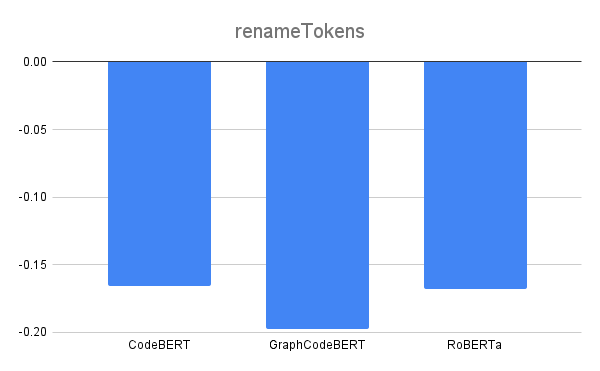
\includegraphics[width=0.20\textwidth]{figs/renameTokens.png}
    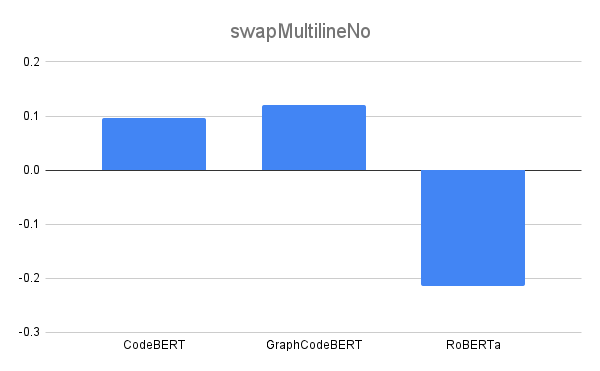
\includegraphics[width=0.20\textwidth]{figs/swapMultilineNo.png}
    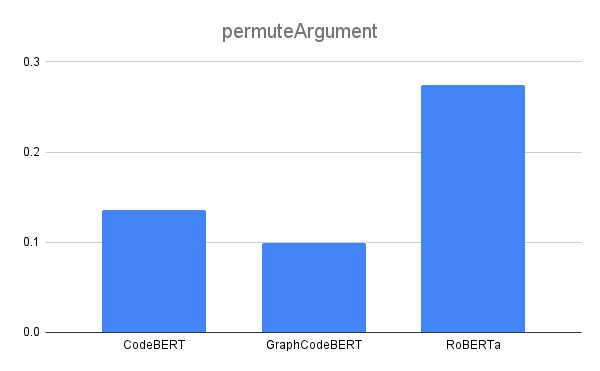
\includegraphics[width=0.20\textwidth]{figs/permuteArgument.png}
    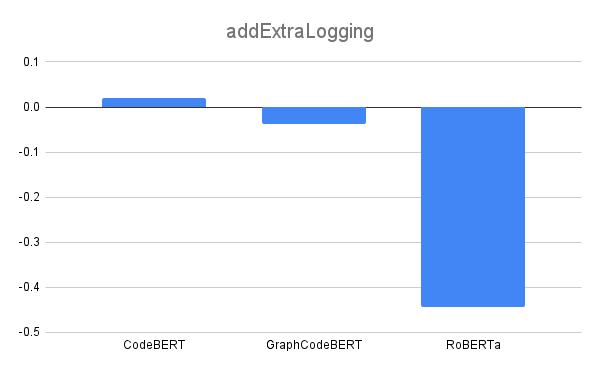
\includegraphics[width=0.20\textwidth]{figs/addExtraLogging.png}
    \caption{Average relative difference across all models.}
    \label{fig:dataflow}
  \end{figure}

  In both cases, we observe a clear trend across method complexity: SCTs in low complexity code have a larger effect on completion quality than similar transformations in high-complexity code. We hypothesize this phenomenon can be explained by the fact that the same transformation can have a comparatively larger effect on a shorter code snippet than a longer one, which contains more contextual information and is thus more stable to minor perturbations.

  Examining the source code transformations, we notice that renaming can have a significant effect on document synthesis. As the model frequently copies tokens from the source code to the document and vis-versa, renaming tends to have a deleterious effect on document quality. Likewise, swapping multiline statements appears to have a significant negative effect on document quality.

  \section{Conclusion}\label{sec:conclusion}

  The work described herein is primarily an empirical study, but also showcases a framework and a systematic approach to evaluating neural code completion models. It offers a number of advantages from a software engineering standpoint: due to its functional implementation, it is efficient, parallelizable and highly modular, allowing others to easily reuse and extend our work with new benchmarks.

  Despite its simplicity, the regex-based SCT approach has some shortcomings. Although regular expressions are easy to implement and do support rudimentary transformations, they are a crude way to manipulate source code. In order to generate semantically valid transformations, one must really use full-fledged term rewriting system, such as higher-order abstract syntax or some kind of parser-combinator. Several options were evaluated, including OpenRewrite, TXL~\citep{cordy2004txl}, Refal~\citep{gurin1991refal} et al., but their features were ultimately found wanting (e.g., poor error recovery) and the complexity of using them (e.g., parsing, API integration) proved too burdensome.

  Our SCTs can be viewed as ``possible worlds'' in the tradition of modal logic: the original author plausibly could have chosen an alternate form of expressing the same procedure. Although we are unable to access all these worlds, we can posit the existence and likelihood of some, and given a dataset of alternate code snippets, begin to probe a candidate model's predictions.

   One intriguing avenue for future work would be to consider combinations of source code transformations. This would vastly expand the cardinality of the validation set, enabling us to access a much larger space of possible worlds, albeit potentially at the risk of lower semantic admissibility, as arbitrary combinations of SCTs can quickly produce invalid code. This presents an interesting engineering challenge and possible extension to this work.

  Although we currently only use average mutlimask accuracy and ROUGE-synonym metrics, it would be useful to incorporate various other metrics such as mean average precision (MAP), mean reciprocal rank (MRR), and normalized discounted cumulative gain (NDCG). In addition to their utility as yardstick for evaluating model robustness, these metrics can be used to retrain those same models, a direction we hope to explore in future work.

  Finally, one could imagine using the code completion model itself to generate code for testing the same model. We have implemented this functionality to a limited extent in the \lstinline|addExtraLogging| SCT, in which the model synthesizes a single token to log, and the \lstinline|insertComment| SCT, where the model inserts a short comment. While this approach could be a useful way to generate additional training data, it would would require careful monitoring and postprocessing to avoid introducing unintended feedback loops.

  Neural language models hold much promise for improved code completion, however complacency can lead to increased reviewer burden or more serious technical debt if widely adopted. While trade secrecy may prevent third-party inspection of pretrained models, users would still like some assurance of the model's robustness to naturally-occurring variance. Our work helps to address this use case, treating the model as a black box: it does not require direct access to the model parameters or training data.

  Our contributions in this work are twofold: we demonstrate that SoTA neural language models for source code, despite their effectiveness on long-range sequence prediction tasks, are unpredictable in the presence of specifically-constructed cosmetic variation. We also describe a systematic approach and open source implementation of a newly-developed software toolkit which allows users to empirically probe a candidate model's robustness to various categories of syntactic and semantic source code transformations.
  \pagebreak\bibliography{main}
  \bibliographystyle{plain}
  \appendix


\end{document}
\endinput